\documentclass[12pt]{article}
\usepackage{graphicx} % Required for inserting images

\title{Lab 4: Alpha Spectroscopy and Range Measurement}
\author{Owen Strong \\
\itshape Prof.: Angela DiFulvio\\
\itshape TA: Kholod Mahmoud \\
\itshape TA: Shaffer Bauer \\
\itshape TA: Justin Jia \\
}
\date{March 5, 2026 (Adjusted from February 28)}

\usepackage[
    style=ieee
]{biblatex}
\bibliography{refs.bib}

\usepackage[letterpaper, margin=1in]{geometry}
\usepackage{xspace}
\newcommand{\figwidth}{0.75\linewidth}

% Common Macros
\newcommand{\figref}[1]{Fig.~\ref{#1}}

% Specific lab to lab
\newcommand{\micCi}{~$\mathrm{\mu Ci}$~}
\newcommand{\AmSrc}{\xspace$^{241}$Am\xspace}
\newcommand{\PoSrc}{\xspace$^{210}$Po\xspace}


\usepackage{placeins} % FloatBarrier
\usepackage{amsmath} % align
\usepackage{xcolor}
\usepackage[colorlinks=true, citecolor=violet, linkcolor=violet, urlcolor=violet]{hyperref}
\usepackage{enumitem}

\begin{document}
\pagenumbering{gobble}
\maketitle
\pagebreak
{\hypersetup{linkcolor=black}\tableofcontents}
\pagenumbering{arabic}
\begin{abstract}

\end{abstract}

\section{Introduction and Background}
A key metric of interest for radiation in matter is range, that is, the depth along the initial direction which a particle is expected, on average, to penetrate through a material.
For a given type of particle, this range is further highly dependent on an incident particle's energy and the electron/neutron densities of the medium.\cite{npre_lab_4_manual_2025}
This laboratory investigates the range of alpha particles, as emitted by \AmSrc and \PoSrc, through aluminum metal, Mylar\footnote{While material names are usually kept in lowercase, ``Mylar'' is a brand name, and remains accordingly capitalized in this report.} plastic, and air.
More broadly, the energy loss phenomena of alpha particles through different materials, including energy straggling, and the effects of geometric attenuation corresponding to solid angle, are also investigated.
\subsection{Charged Particle Energy Loss}



\section{Experimental Procedure}\label{sec:methods}
In this section, we detail the equipment used and experiments performed in this laboratory. Further equipment details may be found in Appendix~\ref{app:equip}
\subsection{Equipment}
In this laboratory, we employed 


\subsection{Range Estimation}
Since particles may not stop at exactly the same distance, to practically estimate the range of the particle and energy, we estimate the range of a particle as the distance where only half the particles are transmitted, as seen in \figref{fig:}
In lieu of exact particle transmission rates, we then estimate this by the distance where peak intensity drops to half that of that measured for the lowest distance.
\section{Experimental Results}\label{sec:results}\FloatBarrier

In \figref{fig:vac_dist_v_I}, the integrated count rate for the alpha source is shown after attenuation through different distances in vacuum. 
However, to does not account for the geometric attenuation, one must first normalize by solid angle $\Omega$, using the following formula\cite{knoll_radiation_2010}:
\begin{equation}\label{eq:sangle}
    \Omega=2\pi\left(1-\frac{d}{\sqrt{d^2+a^2}}\right)
\end{equation}
where $d$ is the distance of the (point) source from the detector, and $a$ the diameter of the detector, a sufficiently long cylinder.
This formula assumes the point source is centered on the cylindrical detector's axis.\\

If the source can ``see'' $\frac{\Omega}{4\pi}$ of the detector, then dividing by this fraction yields an intensity normalized by solid angle.
\figref{fig:vac_dist_v_nI} shows the integrated count rate for distances through vacuum, normalized by solid angle, compared to the original rates.\\

\newcommand{\defplot}[2]{
    \begin{figure}
        \centering
        \includegraphics[width=\figwidth]{fig/#1.png}
        \caption{#2}
        \newcommand{\tmplabel}{fig:#1}
        \label{\tmplabel}
    \end{figure}
}
\defplot{vac_dist_v_I}{The integrated peak intensity of the alpha source after attenuation through varying distances in vacuum.}
\defplot{vac_dist_v_nI}{The integrated peak intensity of the alpha source after attenuation through varying distances in vacuum, both raw and after normalizing by visible solid angle.}

In Figs.\ref{fig:air_dist_v_nI} through \ref{fig:air_dist_v_FWHM}, attenuation over distance in air can be observed through effects on integrated peak intensity (both gross and normalized rates), energy, and full width half maximum (FWHM) of energy peaks.
Normalized peak intensity appears to reach half that of the first measurement between the measurements at 17 and 25 mm, yielding a range estimate of $21\pm4$~mm for 5.486 MeV alpha particles in air. 
\\

\defplot{air_dist_v_nI}{The integrated peak intensity of the alpha source after attenuation through varying distances in air, both raw and after normalizing by visible solid angle.}
\defplot{air_dist_v_E}{The peak energy after attenuation through different distances in air.}
\defplot{air_dist_v_FWHM}{The full width half maximum of peak energy after attenuation through different distances in air.}

The attenuation through aluminum, also shown through effects on peak intensity, peak energy, and peak FWHM, are shown in Figs.~\ref{fig:Al_thick_v_I}, \ref{fig:Al_thick_v_E}, and~\ref{fig:Al_thick_v_FWHM}.
Figs.~\ref{fig:My_thick_v_I}, \ref{fig:My_thick_v_E}, and~\ref{fig:My_thick_v_FWHM} show the same for Mylar.
Intensity appears to halve around 36 microns of aluminum, and with measurements every 18 microns, this yields a range estimate of $36\pm9$~microns in aluminum.
For Mylar, peak intensity drops below half between 7.2 and 10.8 microns, yielding a range estimate of $9.0\pm1.8$~microns.
\\

\defplot{Al_thick_v_I}{The integrated peak intensity after attenuation through varying thicknesses of aluminum.}
\defplot{Al_thick_v_E}{The peak energy after attenuation through varying thicknesses of aluminum.}
\defplot{Al_thick_v_FWHM}{The full width half maximum of peak energy after attenuation through varying thicknesses of aluminum.}

\defplot{My_thick_v_I}{The integrated peak intensity after attenuation through varying thicknesses of Mylar.}
\defplot{My_thick_v_E}{The peak energy after attenuation through varying thicknesses of Mylar.}
\defplot{My_thick_v_FWHM}{The full width half maximum of peak energy after attenuation through varying thicknesses of Mylar.}

\FloatBarrier
Using the simulated data of 5.486~MeV alpha ion transmission in dry air, aluminum, and Mylar in TRIM, rough estimates of total stopping power $-dE/dx$, using an estimate of the derivative between adjacent measurements of energy $E$ and $x$:
\begin{equation}\label{eq:dedx}
    -\frac{-dE_{i+\frac{1}{2}}}{dx_{i+\frac{1}{2}}}\approx\frac{E_i-E_{i+1}}{x_{i+1}-x_i}
\end{equation}
where $E_{i+\frac{1}{2}}=\frac{1}{2}(E_i+E_{i+1})$.
Using equation~\ref{eq:dedx}, estimates of total stopping power $-dE/dx$ can be observed in \figref{fig:air_dEdx} and \figref{fig:My_dEdx}.
For aluminum, TRIM did not calculate any ions being successfully transmitted through more than 1 layer, and so no stopping power estimate could be made this way.\\

\defplot{air_dEdx}{The total stopping power of 5.486MeV alpha particles in air, estimated using energy attenuation at five distances calculated by TRIM.}
\defplot{My_dEdx}{The total stopping power of 5.486MeV alpha particles in Mylar, estimated using energy attenuation at five distances calculated by TRIM.}

\FloatBarrier

Using SRIM, we calculated nuclear, electron, and total stopping powers for alpha particles ranging in energy from 10~keV to 10~MeV.
These are plotted in \figref{fig:air_SRIM} for air, \figref{fig:Al_SRIM} for aluminum, and \figref{fig:My_SRIM} for Mylar.\\

\defplot{air_SRIM}{The nuclear, electron, and total stopping powers of air for alpha particle ions of energies ranging from 10~keV to 10~MeV, calculated using SRIM.}
\defplot{Al_SRIM}{The nuclear, electron, and total stopping powers of aluminum for alpha particle ions of energies ranging from 10~keV to 10~MeV, calculated using SRIM.}
\defplot{My_SRIM}{The nuclear, electron, and total stopping powers of Mylar for alpha particle ions of energies ranging from 10~keV to 10~MeV, calculated using SRIM.}

\FloatBarrier

Likewise, we calculated the projected range of alpha particles with energies ranging from 10~keV to 10~MeV using SRIM.
\figref{fig:air_range} compares these ranges to the range for 5.486~MeV alpha particles in air, while \figref{fig:AlMy_range} compares these for aluminum and Mylar.

\defplot{air_range}{The range of alpha particles between 10~keV and 10~MeV in energy in air, calculated using SRIM, compared to the 5.486~MeV range estimated using experimental attenuation.}
\defplot{AlMy_range}{The range of alpha particles between 10~keV and 10~MeV in energy in aluminum and Mylar, as calculated using SRIM, compared to the 5.486~MeV ranges estimated using experimental attenuation.}

\FloatBarrier

The energy spectra of 5.486 MeV alpha particles transmitted through various distances in air, aluminum, and Mylar can be compared in \figref{fig:combined-spectra}.

\begin{figure}
    \centering
    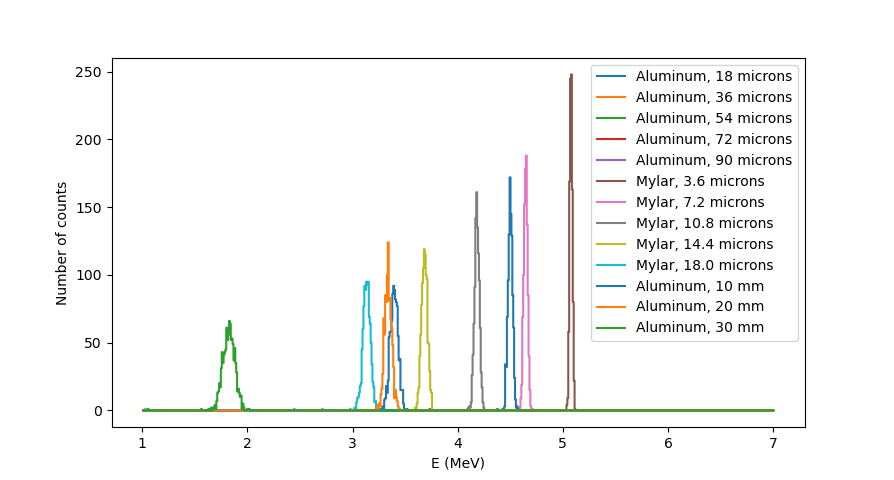
\includegraphics[width=\linewidth]{fig/combined_spectra.png}
    \caption{Energy spectra of 5.486 MeV alpha particles transmitted through various thicknesses of air, aluminum, and Mylar.}
    \label{fig:combined-spectra}
\end{figure}

\FloatBarrier\section{Discussion}\label{sec:disc}
The solid angle calculation of Equation~\ref{eq:sangle} are expected to normalize the intensity measured between measurements with the source different distances away from the detector.
However, this is not what is observed.
In \figref{fig:vac_dist_v_nI}, while normalization makes the ratios between the different distances' integrated intensity less drastic, it does not remove the relationship of these intensities to the distances they were taken at in vacuum, with further distances still resulting in substantially lower peak intensity.
This might result from a lack of a perfect vacuum being drawn, but might also reflect an imperfect accounting for solid angle.
For example, while Equation~\ref{eq:sangle} treats the source as a point source perfectly aligned with the cylindrical detector's axis, it is possible the source is large enough or was far enough off-axis to affect this approximation.\\

The ranges estimated for 5.486~MeV alpha particles using experimental data varied in accuracy.
In \figref{fig:air_range}, we estimate a range in air substantially lower than that calculated by SRIM.
If our solid angle normalization were imperfect in a way that further decreased intensity by distance than we expected, this might result in such an underestimate in range.
The range in Mylar (\figref{fig:AlMy_range}) was also drastically underestimated, but since these measurements were taken at the same distance, solid angle calculations would not account for this error.
Instead, it is still possible that source location shifted more than trivially between measurements, or that wrinkles in the somewhat unwieldy Mylar sheets resulted in greater thickness than expected.
In the same figure, we observe a seemingly more accurate estimation of range in aluminum, but a much more substantial error.
This error reflects a large difference in thickness between different measurements, and suggests we did not have thin enough sheets of aluminum to precisely estimate the range of 5.486~MeV alpha particles in aluminum.\\



\section{Conclusions}\label{sec:conc}

% \bibliographystyle{sty/ieeetran}
\pagebreak\printbibliography

\appendix
\pagebreak
\FloatBarrier\section{Equipment Details}\label{app:equip}
In order to better replicate experiments and identify issues, the details of each equipment piece are recorded in Table~\ref{tab:equip}.

\newcommand{\na}{$N/A$}
\newcommand{\sref}[1]{$^{\ref{#1}}$}
\FloatBarrier
Further details of equipment are listed in Table~\ref{tab:equip}.
Where a detail could not be identified for a given device, it is replaced with ``\na''.
\begin{table}[!h]
    \centering
    \small
    \caption{Details of the equipment used in this laboratory.}
    \label{tab:equip}
    \scriptsize
    \begin{tabular}{c|cccc}
        Item & Manufacturer & Model & ID Type & ID Number\\\hline
        Module rack & Canberra (now Mirion)\sref{addr:mirion}& Model 2000 & Inventory \# & NE759377 \\
        Geiger-Muller Detector & \na & \na & \na & \na \\
        GM Pulse Inverter & Spectrum Techniques\sref{addr:spect} & 2017 GPI & \na & \na \\
        % Multichannel Analyzer & Ortec\sref{addr:ortec} & EasyMCA & Inventory \# & P10F79090 \\
        % Weak Source 1 & Spectrum Techniques\sref{addr:spect} & 1.0\micCi ~$^{137}$Cs Beta Source & Date & Sep. 2017 \\
        % Weak Source 2 & Spectrum Techniques\sref{addr:spect} & 1.0\micCi ~$^{137}$Cs Beta Source & Date & Sep. 2017 \\
        % Strong Source & Eckert and Ziegler\sref{addr:eck-zieg} & 30\micCi~$^{137}Cs$ Beta Source & Date & Sep. 2017 \\
        % \InMeta~Source & \na & Irradiated Indium Foil & Date & Feb. 2026 \\
        High Voltage Power Supply & Caen\sref{addr:caen} & N1470AL & Inventory \# & P10G96054 \\
        % Pulser & Ortec\sref{addr:ortec} & Model 480 & \na & \na \\
        % Oscilloscope & Keysight\sref{addr:keys} & Infiniivision DSO-X 2002A & Inventory \# & P10R03513 \\
        % Counter & Ortec\sref{addr:ortec} & Model 871 & Serial \# & 1024 \\
        % Preamplifier & Ortec\sref{addr:ortec} & Model 142PC & Serial \# & 2780r17 \\
        % Amplifier & Ortec\sref{addr:ortec} & Model 590A & Serial \# & 16076205 \\
        Computer & Dell\sref{addr:dell} & Precision 360 & Eng. IT ID \# & EWS 20426 \\

    \end{tabular}
    \begin{enumerate}[label=\alph*]
        \item\label{addr:mirion}
        Mirion Technologies, Inc.:
        1218 Menlo Drive,
        Atlanta, GA;
        Phone: 770.432.2744;
        \url{https://ir.mirion.com/}
        \item\label{addr:spect}
        Spectrum Techniques:
        106 Union Valley Rd, Oak Ridge, TN 37830;
        Phone: 865.482.9937;
        \url{https://www.spectrumtechniques.com/}
        \item\label{addr:eck-zieg}
        Eckert \& Ziegler Isotope Products:
        24937 Avenue Tibbitts, Valencia, CA 91355;
        Phone: +1 866 476-9767;
        \url{https://isotopeproducts.com/}
        \item\label{addr:caen}
        Caen Sp.A.:
        Via della Vetraia, 11, 55049 Viareggio LU - Italy;
        Phone: +39 0584 388398;
        \url{https://www.caen.it/}
        \item\label{addr:keys}
        Keysight Technologies: 
        1900 Garden of the Gods Road, Colorado Springs, CO 80907-3423 United States;
        Phone: 1 800 829-4444;
        \url{https://www.keysight.com}
        \item\label{addr:ortec}
        Advanced Measurement Technology:
        801 South Illinois Avenue,
        Oak Ridge, Tennessee 37830,
        United States;
        Phone: +1.865.482.4411;
        Fax: +1.865.483.0396;
        \url{https://www.ortec-online.com};
        Email: ortec.info@ametek.com
        \item\label{addr:dell}
        Dell Technologies:
        Dell Technologies
        1 Dell Way
        Round Rock, TX 78664.;
        Phone: 1-877-275-3355;
        \url{https://www.dell.com/en-us/lp/contact-us}
    \end{enumerate}
\end{table}
\FloatBarrier
\end{document}
